\chapter{Implementation Test}
In this chapter, a brief demonstration testing cases are presented. To be more specifically, two testing scenarios related with \emph{CommunicationStack} applet and simulated remote server are designed. At the same time, the testing cases demonstrating communication between Smart Home web server component and Android application are designed.

\section{Remote Management Testing}
The aim of this testing scenario is to prove the feasibility of applying Smart Card and remote application/file management protocols proposed by Globalplatform to provide a secure dual authentication and messaging platform for other 
higher leveled applications. My Javacard Applet, \emph{CommunicationStack} together with correspondingly designed \emph{UTE} test cases are employed together building the testing environment.

\subsection{\emph{UTE} Test Case}

Two \emph{UTE} test cases are programmed. They are:
\begin{itemize}
\item \emph{Trigger Communication Channel with SMS}. In this test case, I simulate the open communication channel process between smart card and remote administrator server. This process is also the cornerstone for a successful remote management.
\item \emph{Secure Messaging Exchanging} After a successful identification between communication peers and creation of communication channel, in this test scenario, smart card and remote server are going to perform secure messaging. 
\end{itemize}

\subsubsection{Trigger Communication Channel with SMS} \label{secAppletTest1}
In this test suit, UTE testing case acts as an OTA server and encapsulates information for the construction of a secure HTTP channel in a \emph{TriggerPushSMS} object and sent this SMS to target smart card applet using simulated GPRS connection.  The whole SMS structure is pictured in figure~\ref{fig:pushSMS} and encapsulated parameters are categorized as following:
\begin{itemize}
\item \emph{Connection Parameters}, which includes network access name, bearer description and other parameters describing the simulated remote server.
\item \emph{Security Parameters} In security parameters, proposed TLS 1.2 connection information, such as suggested cipher suit, is provided
\item \emph{Smart Card Keysets}, that consists of key identifiers as well as indicator used for the select of cipher keys, signature keys.
\item \emph{HTTP connection parameters}. Also parameters such as retry counter, timeout values are included in this short message.
\end{itemize}
After a successful receive and process of aforementioned push SMS, \emph{CommunicationStack} will preform TLS handshake with remote server, in demonstration case \emph{TLS\_PSK\_WITH\_NULL\_SHA256} is applied, and construct HTTP connection using HTTP Header proposed in ~\ref{secHTTPHeader}.

Figure ~\ref{fig:mk} and ~\ref{fig:verify-pass} shows a successful creation of secure channel between remote server and smart card applet.

\begin{figure}[!htp]
	\centering
	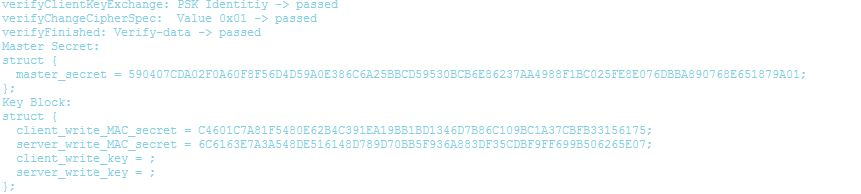
\includegraphics[width=1.1\textwidth]{Images/impl/mk.jpg}
		\caption{Successful generation of master key between remote server and \emph{CommunicationStack} applet}
	\label{fig:mk}
\end{figure}

\begin{figure}[!htp]
	\centering
	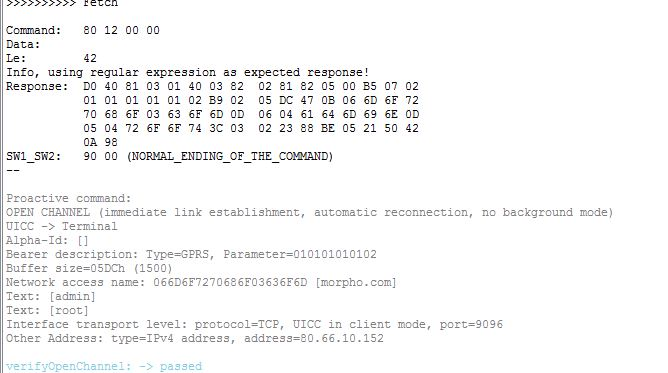
\includegraphics[width=1.1\textwidth]{Images/impl/verify-pass.jpg}
		\caption{Successful creation of secure channel}
	\label{fig:verify-pass}
\end{figure}

\subsubsection{Secure Messaging Exchanging}
Based on in previous paragraph ~\ref{secAppletTest1} created secure channel and HTTP Connection, in this test case, smart card applet and remote server performs message exchanging. Demonstration configuration parameters are already given in section z

\section{Android Application Testing}